\section{Unstrukturiertes Gitter}
Um den Unterschied zwischen einem strukturierten und unstrukturierten Gitter festzustellen, wurden zusätzlich Berechnungen mit einem unstrukturierten durchgeführt. Diese Berechnungen konnten aufgrund einiger aufgetretener Probleme nicht hinreichend betrachtet werden.

\subsection{Aufgetretene Probleme}
Für den zweiten Stator liegt keine Geometrie, lediglich ein Netz vor. Somit war es nicht möglich ein unstrukturiertes Gitter für diesen zu erstellen. Für die Berechnungen wurde daher die Aachen-Turbine teilweise unstrukturiert und strukturiert betrachtet.\\
Ein weiteres Problem stellt die Ausrichtung der ersten Stufe da.
Bei dieser muss das Gitter verschiedene Transformationen durchlaufen:
\begin{itemize}
\item Rotation um die y-Achse um $90^\circ$
\item Rotation um die x-Achse um $180^\circ$
\item Spiegelung der Schaufel an der x,z-Ebene
\item Translation des zweiten Stators entlang der z-Achse
\end{itemize}
Weiterhin lassen sich einige Punkte aus dem Setup des strukturierten Gitters durch die durchgeführten Transformationen nicht verwenden, da diese außerhalb des Rechengebiets liegen.\\
Die Erstellung der unstrukturierten Gitter war aufgrund von Lizenzproblemen nicht immer möglich, was die Anzahl der durchgeführten Simulationen eingrenzt.
\subsection{Erstellung des Gitters}
Das unstrukturierte Gitter wurde mit Centaur erstellt. Zunächst wurde ein Referenzgitter mit den Defaultwerten gebildet. Für das Einstellen von $y^+$ wurde in einem ersten Test der gleiche Wandabstand wie im Falle des strukturierten Gitters verwendet. Nach einem ersten Test wurde dieser im Rotor verringert. Die Verteilung von $y^+$ des ersten Stators und Rotors ist in Abbildung \ref{yplusunstrukturiert} dargestellt.
\begin{figure}[htbp]
	\centering
	\includegraphics[width=0.7\textwidth]{yplusunstrukturiert.png}
	\caption{$y^+$ des unstrukturierten Gitters} \label{yplusunstrukturiert}
\end{figure}
\subsubsection{Verwendung von Sources}
Um das Gitter lokal an bestimmten Stellen zu verfeinern wurden sogenannte Sources in Centaur eingeführt.
Eine davon regelt den unterschiedlichen Wandabstand von Blade zu dem von Hub, beziehungsweise Shroud.\\
Eine Weitere verfeinert die Zellen im Nachlauf der Schaufel relativ um den Faktor $c = 0.8$

\subsection{Gitterstudie}
Zuerst wurde der Spalt des Rotors wie beim strukturierten Gitter verfeinert. Anschließend wurde eine Gitterstudie mit verschiedenen Verfeinerungsstufen, siehe Tabelle \ref{tab:verfeinerungenunstrukturiert}, durchgeführt. In den Abbildungen \ref{fig:gitterunstrukturiert1stufe} und\ref{fig:gitterunstrukturiert15stufen} ist zu erkennen, dass die Wirkungsrgrade weiterhin in Abhängigkeit der Kontrollvolumenzahl steigen. Damit eine netzunabhängige Lösung ermittelt werden kann, müssten weitere Verfeinerungsstufen zwischen 2 und 3 und größer 3 gerechnet werden, bis kein Anstieg oder Absinken mehr zu erkennen ist. Dies war aufgrund von Lizenzproblemen bei Centaur nicht möglich.\\
Für die Berechnungen mit einem temperaturabhängigen $c_p$ und für die Vergleiche mit dem strukturierten Gitter wurde das feinste Netz verwendet.
\begin{table}[h]
		\centering
		\caption{Verfeinerungsstufen des unstrukturierten Gitters}
	\begin{tabular}{ c| c | c| c| c}
Verfeinerungsstufe	&	Stator 1	&		&	Rotor	&		\\
&	Anzahl Knoten	&	Anzahl Elemente	&	Anzahl Knoten	&	Anzahl Elemente	\\
\hline									
0,5	&	61435	&	174098	&	281782	&	724470	\\
1	&	147399	&	473211	&	638948	&	1741931	\\
2	&	244772	&	880367	&	1007020	&	2835297	\\
\textbf{3}	&	\textbf{1196277}	&	\textbf{6457352}	&	\textbf{1880370}	&	\textbf{6844537}	\\

	\end{tabular}
		\label{tab:verfeinerungenunstrukturiert}
\end{table}
\begin{figure}[htbp]
	\centering
	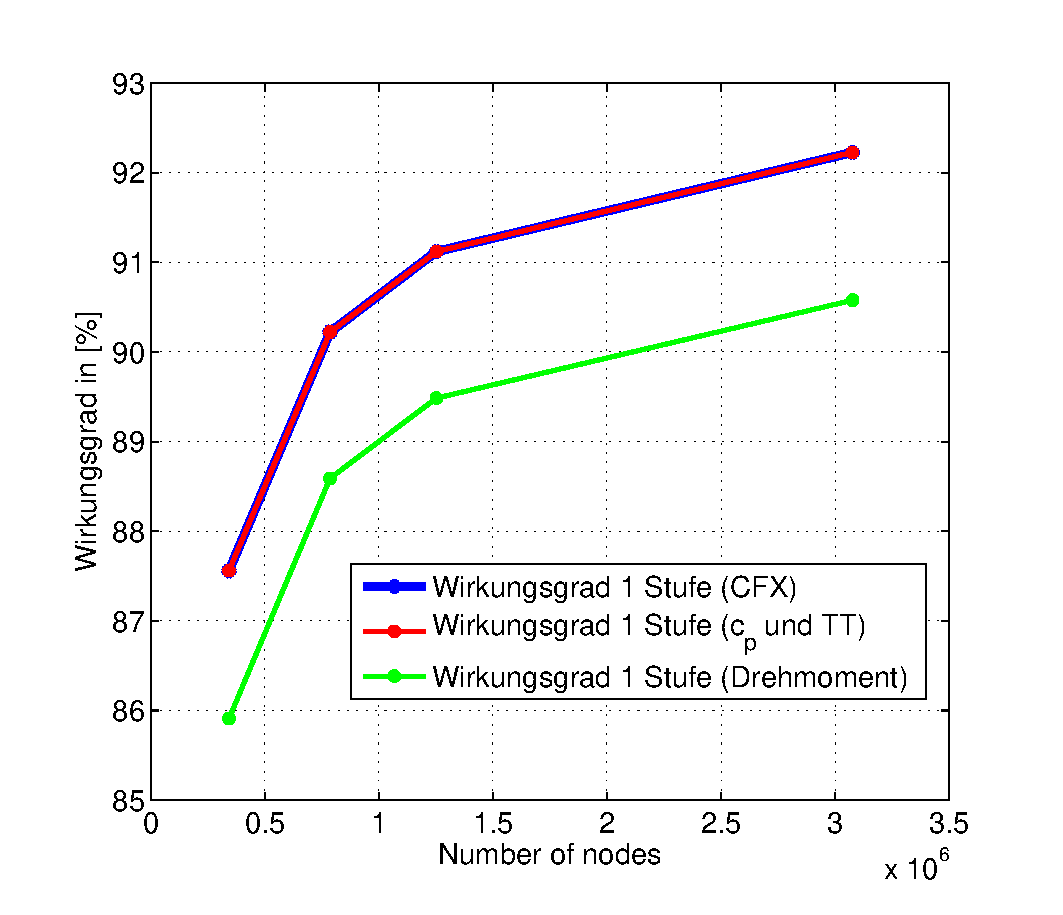
\includegraphics[width=0.7\textwidth]{gitterstudieunstrukturiert1stufe.eps}
	\caption{Gitterstudie des unstrukturierten Gitters für eine Stufe} \label{fig:gitterunstrukturiert1stufe}
\end{figure}

\begin{figure}[htbp]
	\centering
	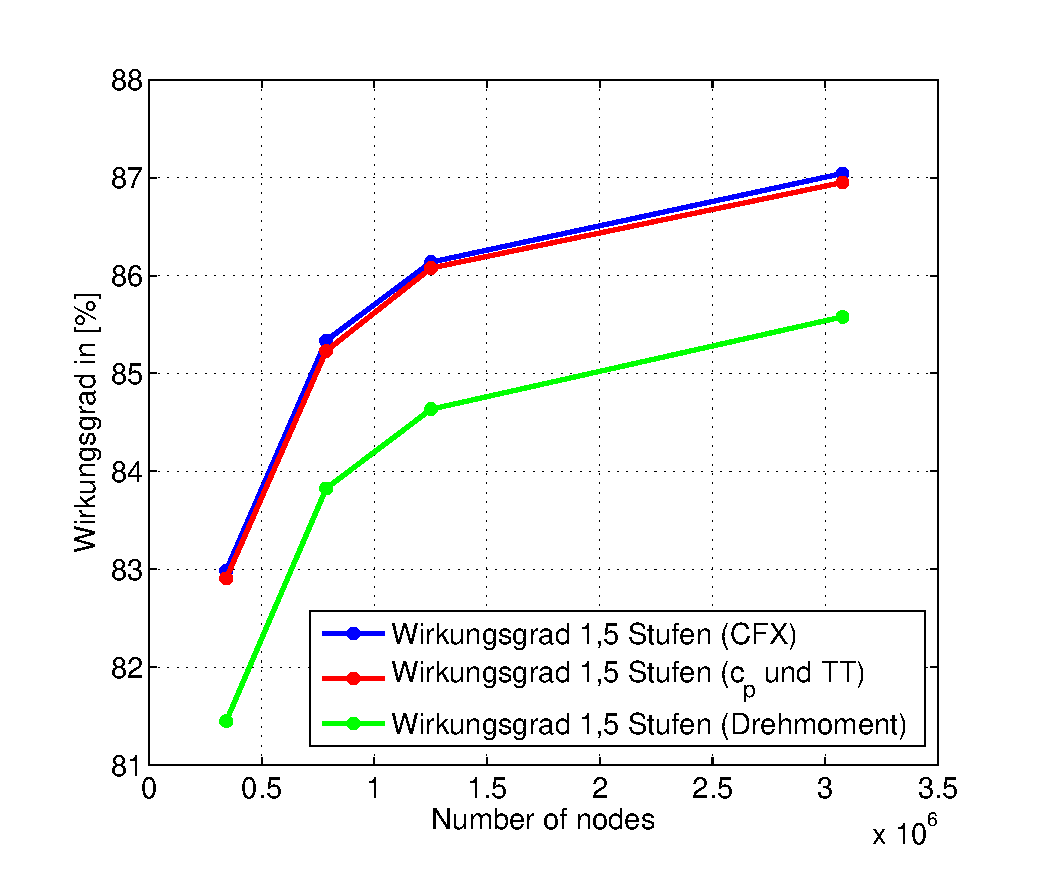
\includegraphics[width=0.7\textwidth]{gitterstudieunstrukturiert15stufen.eps}
	\caption{Gitterstudie des unstrukturierten Gitters für eine Stufe}
	\label{fig:gitterunstrukturiert15stufen}
\end{figure}

\subsection{Temperaturabhängiges $c_p$}
\begin{table}[H]
	\centering
	\caption{Vergleich der Wirkungsgraddefinitionen mit $c_p = f(t)$}
	\begin{tabular}{ l| c | c c c c}
	&	$c_p = const.$	&	$c_p(t)$	&		&		&		\\
	\hline
	&		&	CpIs	&	Ave CpIS	&	Ave	&	mycp	\\
	\hline
CFX	&	80,21 \%	&	71,93 \%	&	77,96 \%	&	78,34 \%	&	60,01 \%	\\
$c_p$ und $T_t$	&	80,1 \%	&	\textcolor{red}{100,36} \%	&	78,23 \%	&	78,61\%	&	83,72 \%	\\
Torque	&	79,5 \%	&	70,23 \%	&	77,1 \%	&	77,48 \%	&	59,36 \%	\\

	\end{tabular}
	\label{tab:unstrukturiertmycp}
\end{table}